\chapter{绪论}

\section{课题来源}
本课题来源于长春国科精密光学技术有限公司的横向项目:“激光测长干涉仪研制”(课题编号 KCH2310069)。

\section{研究背景及意义}
随着信息技术和数字经济的不断发展,半导体技术及集成电路产业不断高歌猛进,已广泛应用于消费电子、医疗电子、通信产业、汽车工业和国防事业等领域,是一个国家科技水平高低的重要标志之一,也是我国经济发展和国防安全的支柱产业。中国半导体行业协会(China Semiconductor Industry Association,简称CSIA)的相关数据显示,我国的集成电路产业稳步成长,在2021年度行业的销售额首次突破万亿大关,达到10458.3亿元,同比增长18.2$\%$,2022年度仍然保持着的良好的增长速度,2022上半年的销售额达到4763.5亿元,同比增长16.1$\%$\cite{csia1}。而半导体设备是半导体行业的基石,根据国际半导体产业协会(简称SEMI)的相关数据显示,中国已经成为全球最大的半导体市场,在2021年度半导体设备的销售额已经达到1026亿美元,同比激增44$\%$\cite{中国再次成为全球最大半导体设备市场}。而我国也早已开展半导体设备的相关研发工作,以光刻机中的核心系统——投影物镜为例,在十三五期间就已进行了单独立项研究(项目编号:2016ZX02201001)。

为了补偿波像差,光刻机中的投影物镜系统需要同时使用多个可以调节的驱动镜片,并且实现闭环反馈控制,这对位移传感器的精度有了较大的依赖;同时,随着半导体尺寸的不断减小,对于芯片制造商而言,时间就是金钱,所以为了适应光刻机产率的提高,掩模台和硅片台的运动速度也不断增大,如今已经达到了3m/s,并且以先进的EUV光刻机(NXE:3400C,ASML)为例,其吞吐量可以达到170片/小时,在光刻机如此高产率的前提下仍然要保持位移传感器的正确率,这对位移传感器的测量速度提出了新的挑战;而近几年来大尺寸电子设备的显示需求的增加也导致了光刻机的测量尺寸和运动行程越来越大,这导致对位移传感器的量程提出了很高的要求。综上所述,由于半导体技术的不断发展,对位移传感器提出了亚纳米级分辨率、纳米级测量精度、数米级的测量速度和米级的测量量程等要求。在光刻机对位移传感器有着如此高要求的前提下,国外的很多知名公司(如Heidenhain公司)在超高精密测量领域并不对中国提供定制化的高精度传感器,而国内也仅有部分高校研制出了原理样机,距离实用还有一定距离,在此情形下,自主研发高精度的位移传感器已经迫在眉睫。当前比较常见的高精度位移传感器主要有电容位移传感器、光栅尺以及双频激光干涉仪,相关文献和研究者的研究工作表明双频激光干涉仪能满足上述的测量需求\cite{2022reso1ution,张志平2022激光外差干涉技术在光刻机中的应用,于海娇2022双频激光干涉仪的应用研究综述,2007Studyon,2021Microchip,202019picometer}。

电容传感器的原理是将位移等物理量的变化情况以电容的变化反映出来,传感器的敏感元件是由一个参数可变的电容构成的,主要由上下极板、绝缘介质和衬底组成,当由于位移等物理量变化使得上下极板之间的相对距离、相对面积或者绝缘介质的介电常数发生变化时\cite{孙凤鸣2013基于},电容值也会发生变化,然后由电容检测电路检出。但由于电容传感器结构和体积的限制,其电容一般只能达到皮法量级,有的甚至只能达到飞法量级,这会给电容检测电路带来很大困难,并且由于电容检测电路的非线性使得传感器的测量曲线线性度不好,但电容的微小值使得其在微小位移检测上具有较大优势\cite{Maya2019Low,2015Ahighprecisio,王晓立2011电容式位移传感器研究}。目前市面上高精度的电容传感器供应商主要为美国的MTI公司和德国的米铱公司,而我国对于电容位移传感器的研究起源于20世纪70年代,起步较晚,目前的产品普遍量程较小,分辨率较低\cite{曹妍0基于膜电极的电容微位移传感器研究与设计}。


纳米级光栅尺的基本原理主要是利用在入射光源照射下,标尺与光栅扫描图像掩模之间的相对运动形成的莫尔条纹,莫尔条纹通过多个光电探测器转换,变成近似正弦波和余弦波的光电信号,然后反推出位移值\cite{1999Study}。光栅尺由于具有较短的光路,使其对环境具有一定的鲁棒性\cite{,2021Real},但是光栅间距一般为2μm或0.5μm\cite{2020CPLD},并且光栅间距的均匀性会严重影响光栅尺测量的重复测量精度,这对光栅的制造工艺是个挑战。并且大长度、高线数的光栅尺制造较为困难,这导致光栅尺较难保障高测量分辨率的前提下做到较大的测量量程\cite{苏绍璟2001大量程纳米级光栅位移测量理论及关键技术研究}。目前市面上高精度的光栅尺主要由德国的Heidenhain公司提供。

激光干涉仪分为单频(零差式)激光干涉仪和双频(外差式)激光干涉仪,单频激光干涉仪受光强波动的影响较大,鲁棒性较差,而双频激光干涉仪将直流信号转换为交流信号进行测量,抗干扰能力强、对光强波动不明显。市面上的双频激光干涉仪均以氦氖双频激光器为光源,采用迈克尔逊干涉技术实现长距离纳米级测量精度,它可以追溯到米的基准定义,所以测量结果非常可信,它是最权威的线性测量和在线测量仪器\cite{NovelWay}。美国国家标准技术局研制的“校准式原子力显微镜”中就含有双频激光干涉仪,精度可达0.1nm。我国也于20世纪70年代就开始了激光干涉仪的研究\cite{楚兴春2005纳米光栅干涉位移测量关键技术的研究},目前哈工大光电所的D150激光干涉仪的测量分辨率已达到亚纳米级别\cite{马磊2018星间激光干涉仪测距技术发展现状与趋势}。而双频激光干涉仪的最大测量速度如式\eqref{eq:干涉仪最大测量速度}所示\cite{NovelWay},$\Delta f$为激光的频差,通常在几十到几百MHz量级,$\lambda$为激光波长,通常在几百纳米量级,两者相乘其结果很容易达到米级。

\begin{equation}\label{eq:干涉仪最大测量速度}
  v_{max}=\frac{1}{2}\Delta f\lambda
\end{equation}

综上所述,双频激光干涉仪满足亚纳米级分辨率、纳米级测量精度、数米级的测量速度和米级的测量量程等测量要求,或是最适合用于半导体设备的位移测量系统中的产品之一。但是由于双频激光干涉仪的位移测量是以真空环境下的激光波长为基准的,而激光波长跟空气折射率息息相关,而空气折射率容易受到温度、气压等环境因素的影响,这通常会使得实际测量环境下的激光波长小于真空环境下的波长\cite{戴成睿硕士论文面向激光追踪测量系统的空气折射率补偿方法研究},从而对测量产生误差。根据相关文献的描述\cite{徐建2013双频激光干涉仪系统线性测量误差主要来源及减小误差的方法分析} , 在对上述环境因素不进行任何控制或补偿的情况,空气折射率的变化可能会达到 50ppm,如果仅对测量环境温度进行控制,其余因素的变化也可能导致空气折射率变化20ppm以上,这会严重影响双频激光干涉仪的测量精度,而光刻机等半导体设备对位移传感器的精度要求极高,所以急需对双频激光干涉仪的环境误差进行补偿,而且需要尽可能提高补偿精度。



\section{国内外研究现状}
目前常见的补偿空气折射率的方法主要分为两类:直接测量法和间接测量法。光的干涉现象是与波长紧密关联的,利用干涉的某些特点就可以从结果直接反推出空气折射率,这种方法称为直接测量法,例如荷兰爱因霍芬科技大学使用的抽气法、波长跟踪器等。而间接测量法又可以称为PTF法\cite{高精度空气折射率测量系统设计与实现},是利用对应的传感器间接测量出环境的温度、气压、湿度等影响空气折射率的因素,然后使用经验公式计算出空气折射率,常见的方法有Edlen公式、Birch公式等,Edlen公式补偿方法已广泛用于激光干涉仪的环境误差补偿。

\subsection{直接测量法}
1988年英国国家物理实验室的Birch K P等人使用抽气法进行空气折射率的测量,测量光路共分为两部分:真空腔中心管和外管,其中真空腔与气泵相连。入射光经分光镜后产生两束测量光,分别进入真空腔的中心管和外管,随后汇聚产生干涉,利用气泵进行抽气和放气,周期性地改变真空腔中心管的真空度,使其空气折射率发生改变,利用光电探测器记录下干涉信号,并解调出信号的相位差值,从而反推出空气折射率。实验结果表明,在不考虑水蒸气的情况下,该测量方法的测量值与Edlen公式的计算值误差均在$\pm$3.2$\times 10^{-8}$的测量不确定度范围内\cite{1988The}。

2003年,清华大学的陈强华等人提出了一种基于等效合成波方法的空气折射率测量方法,即使用两个长度不同的真空管构成两个虚拟波,从而实现双波长测量,并使用合成理论求解合成波长从而实现空气折射率的测量\cite{2004基于等效合成波方法的双真空管空气折射率测量仪}。实验结果表明,与Edlen公式相比,其测量精度好于1$\times 10^{-7}$,并且具有较好的抗干扰能力,并且结构小巧,使用方便。

Agilent公司设计的10717A的波长跟踪器示意图如图\ref{fig:Agilent 10717A波长跟踪器示意图}所示\cite{羡一民2015折射率修正技术——激光干涉仪技术综述之四},使用的是迈克尔逊干涉仪形式,标准具使用微晶玻璃制造,微晶玻璃受温度等环境因素的影响较小,并且标准具已经在工厂中进行了真空预对准,为此标准具能够保证一个较为固定的光程,作为波长跟踪的基准;而干涉仪的另外一臂暴露在空气中,当温度等环境因素变化时,会使得该臂的光程长度发生变化,产生干涉后将结果与标准具进行对比,即可以得到折射率相对于初始折射率的变化情况,并作为折射率修正的依据。10717A波长跟踪器的精度为0.14ppm。
\begin{figure}[htb]
  \centering
  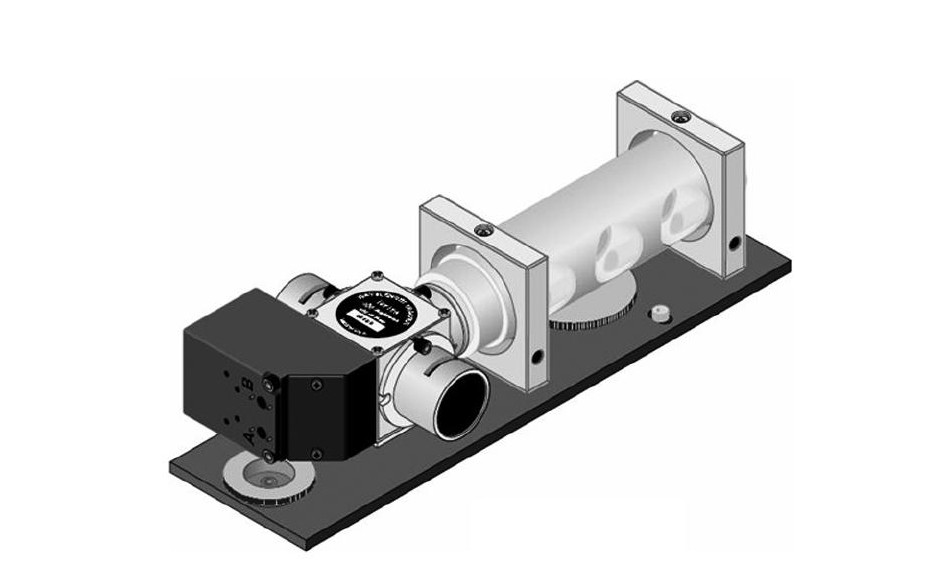
\includegraphics[width=9cm]{fig/1-fig/Agilent 10717A波长跟踪器.jpg}
  \caption{Agilent 10717A波长跟踪器示意图}
  \label{fig:Agilent 10717A波长跟踪器示意图}
\end{figure}

2014年清华大学的池峰等人设计了一种新型的波长跟踪器,具有结构简单、制造成本低等特点,如图\ref{fig:新型波长跟踪器示意图}所示\cite{池峰2014双频激光干涉测量中的环境补偿技术}。该波长跟踪器本质上也是一个激光干涉仪,将干涉仪和被测物镜固定在一个零膨胀底板上,由于底板的热膨胀系数很小,所以其长度几乎不随温度等环境因素变化,所以它能提供一个“标准腔长”(长度200mm),因此通过波长跟踪器测量到的光程变化可以认为全部是由环境折射率变化所导致的,由此可以计算出环境的折射率变化和波长变化,对测量值进行补偿。经过实验验证,在光程长度为200mm时,使用该波长跟踪器进行补偿后,测量误差的3$\sigma$值由24.4nm下降到6.9nm;光程长度为1000mm时,测量误差的3$\sigma$值由109.7nm下降到25.8nm,补偿效果明显,目前该波长跟踪器已成功应用于90nm光刻机中。
\begin{figure}[htb]
  \centering
  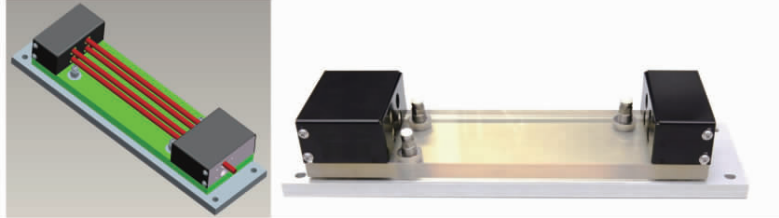
\includegraphics[width=11cm]{fig/1-fig/池峰波长跟踪器.jpg}
  \caption{新型波长跟踪器示意图}
  \label{fig:新型波长跟踪器示意图}
\end{figure}

2017年Yang等人提出了一种光学频率梳校准的扫频干涉法测量空气折射率。当快速扫描可调谐外腔半导体激光器(ECDL)时,通过窄带带通(BP)滤波器从带有频率梳的拍信号生成校准标记,利用实时的激光频率校准标记和两束光束通过双间隔玻璃盒内外区域的干涉信号,可以得到激光频率与干涉位相之间的关系,用于计算空气折射率,实验示意图如图\ref{fig:光学频率梳校准的扫频干涉法测量空气折射率实意图}所示\cite{2017Frequency}。实验结果表明,连续测量空气折射率2h,测量结果相比于Ciddor方程的误差小于9.6$\times 10^{-8}$,标准偏差为5.9$\times 10^{-8}$,空气折射率测量的相对不确定度为8.6$\times 10^{-8}$,测量原理和结构简单,结构紧凑,易于操作,一次完整的测量只需要5s。
\begin{figure}[htb]
  \centering
  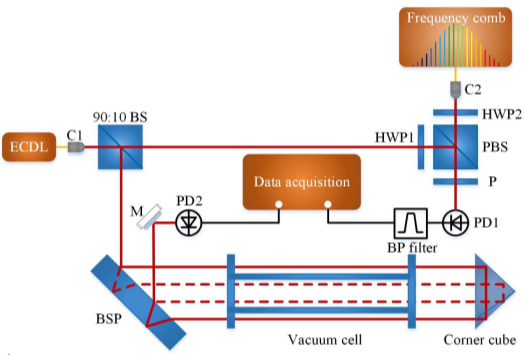
\includegraphics[width=9cm]{fig/1-fig/光学频率梳校准的扫频干涉法测量空气折射率实意图.jpg}
  \caption{光学频率梳校准的扫频干涉法测量空气折射率实意图}
  \label{fig:光学频率梳校准的扫频干涉法测量空气折射率实意图}
\end{figure}

2019年,Chen B等人提出了一种基于变长真空腔调相零差干涉仪测量空气折射率的新方法,通过改变真空腔长度使得空气环境和真空环境之间产生连续的光路变化,并用PGC-Arctan解调方法对干涉仪的相位变化进行解调。该方法最大的优点是能够对振动和空气波动有较强的鲁棒性,在这种情况下也能准确地计算出真空腔长度改变过程中的积分条纹,从而精确解调真空腔长度改变前后的相位。测量装置示意图如图\ref{fig:基于变长真空腔调相零差干涉仪的空气折射率测量装置示意图}所示\cite{2019Precision},M1为参考镜,固定在压电驱动器(PZT)上,M2为被测镜,一个具有固定腔长(W1)和可变腔长(W2)的真空腔放置在PBS和M2之间,W2被放置在一个工作台上,在测量过程中可以移动以改变腔长,PC用于计算信号的相位,MC是运动控制器,用于控制工作台的移动,该方法在实验中与Edlen公式的结果进行了对比,验证了方法的可行性,实验结果表明,其标准偏差在20min内优于2.6$\times 10^{-8}$,在8.5h内优于4.6$\times 10^{-8}$。
\begin{figure}[htb]
  \centering
  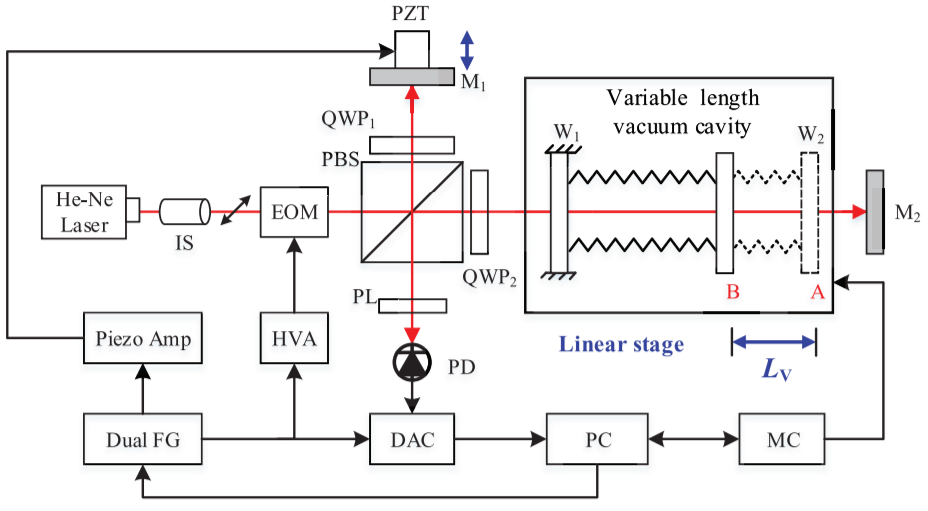
\includegraphics[width=11cm]{fig/1-fig/基于变长真空腔调相零差干涉仪的空气折射率测量装置图.png}
  \caption{基于变长真空腔调相零差干涉仪的空气折射率测量装置示意图}
  \label{fig:基于变长真空腔调相零差干涉仪的空气折射率测量装置示意图}
\end{figure}


\subsection{间接测量法}
2000年,美国的Okafor A C和Ertekin Y M使用Renishaw的低功耗氦氖激光器校准单元以及环境控制器单元(EC10)对立式加工中心(Vertical Machining Center,VMC)的温度变化误差进行精度表征,如图\ref{fig:Sabre 750 VMC 布局和温度传感器位置示意图}所示\cite{2000Vertical}。三个材料温度传感器磁性连接到X轴(左侧)、Y轴(背面)和Z轴电机外壳上,除此之外,气压和湿度传感器探头一起磁性地附着在机器工作台上,用于监测环境影响,而气压和湿度传感器本体位于环境控制器单元 (EC10) 内。上位机Gateway 2000使用EC10的实时传感器输出,使用Edlen公式自动计算获取的激光数据的环境补偿值。
\begin{figure}[htb]
  \centering
  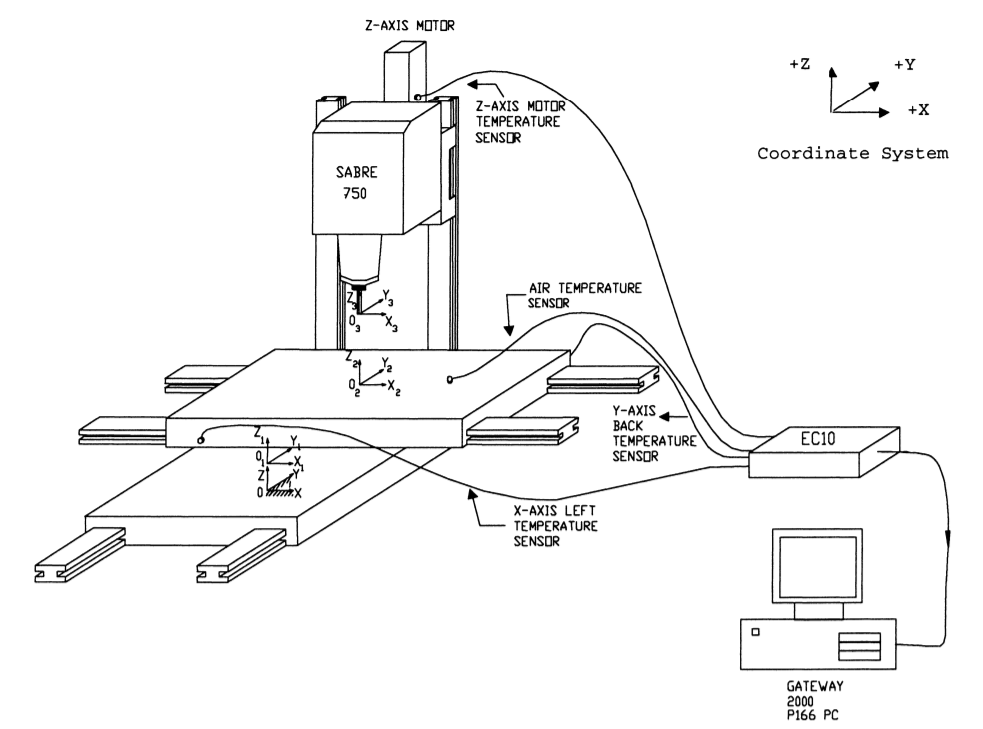
\includegraphics[width=10cm]{fig/1-fig/EC10.jpg}
  \caption{Sabre 750 VMC布局和温度传感器位置示意图}
  \label{fig:Sabre 750 VMC 布局和温度传感器位置示意图}
\end{figure}

由于间接补偿法依赖于Edlen公式进行空气折射率的计算,但是该公式是经验的,并不完全准确,为了提高重复测量精度,满足光刻机等超精密平台对重复定位精度的高要求,2012年GAO等人在Birch和Down修正的Edlén公式的假设的基础上,推导了采用间接补偿法时环境参数的重复测量精度与重复性之间的关系,举例分析了Bonsch的修正公式与Down的修正的Edleen公式之间的差异,说明了该假设的合理性。仿真结果说明,使用Edlen公式的间接补偿法可以达到亚纳米级别的重复测量精度。

2015年,上海市计量测试技术研究院的周毅冰等人为保证激光干涉仪的测量准确度,设计了一套用于激光干涉仪环境误差补偿单元中气压传感器的检定装置,如图\ref{fig:周毅冰等人设计的压传感器的检定装置图}所示\cite{周毅冰2015激光干涉仪环境补偿单元气压传感器检定装置},主要包括气压密封罐、压力控制器和计算机终端三部分。所用的气压传感器的精度等级属于0.1级(根据JJG1084-2013),压力空气制的量程为0-350kPa,气压密封罐的泄露速率在控制器的可控范围之内。实验数据表明, 其重复性和稳定性良好, 整套装置符合JJG1084-2013要求,可用于激光干涉仪的环境误差补偿单元。
\begin{figure}[htb]
  \centering
  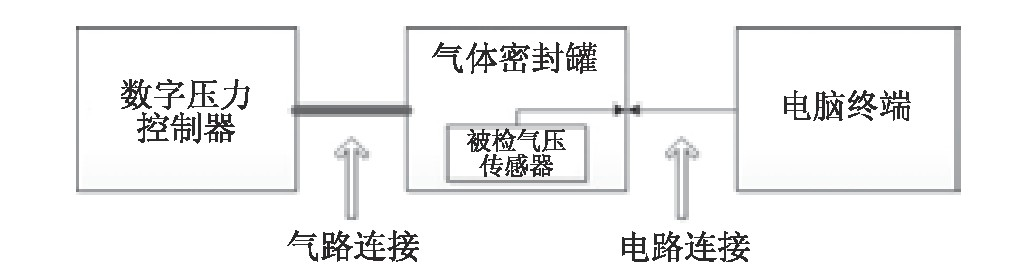
\includegraphics[width=11cm]{fig/1-fig/周毅冰等人设计的压传感器的检定装置图.jpg}
  \caption{周毅冰等人设计的压传感器的检定装置图}
  \label{fig:周毅冰等人设计的压传感器的检定装置图}
\end{figure}

2016年,韩国的K. Lee等人提出了一种使用拉格朗日乘数法对双频激光干涉仪的环境误差进行补偿,即使用拉格朗日乘数法来最小化目标函数,在约束条件下寻找最优解。如式\eqref{eq:拉格朗日乘数法}和式\eqref{eq:拉格朗日乘数法1}所示\cite{2016Lagrange},式中$\Phi$代表理想情况下的的无噪声相位;$I_{x}$和$I_{y}$是包含相位信息$\Phi$的强度信号,a、h、b和v是用于表示环境误差模型的不确定性参数,采用最小二乘法进行估计。实验使用电容位移传感器进行纳米级的测量,结果表明该方法相比于使用最小二乘法进行估计,有着更小的均方根值误差。
\begin{equation}\label{eq:拉格朗日乘数法}
  \tilde{I}_{x} \propto (\frac{AB}{2} + \Delta \alpha)cos \Phi + h = aI_{x} + h.
\end{equation}

\begin{equation}\label{eq:拉格朗日乘数法1}
  \tilde{I}_{y} \propto (\frac{AB}{2} + \Delta \beta) cos \Phi + v = bI_{y} + v.
\end{equation}

2018年,天津大学的吴炳阳等人提出一种利用气压传感器和二等标准铂电阻温度计对数字传感器测量值进行校准和修正的方法, 并利用温度值对大气压值进行修正\cite{吴炳阳2018小型化空气折射率测量装置的精度修正}。该方法使用瑞Sensirion公司SHT75数字式温湿度传感器,温度的精度为$\pm0.3^{\circ}\mathrm{C}$, 相对湿度的精度为$\pm1.8\%$;气压传感器为美国Measurement Specialties Inc公司的Ms5803传感器,测量范围为10-1300hPa, 精度水平为$\pm$1.5hPa。校准后实现标定好长度的真空管,测量出抽真空前后光程长度的变化值,并以此计算空气折射率值。实验结果表明,使用该方法修正后的空气折射率测量值精度为$10^{-8}$,准确度估计等级达到$10^{-7}$量级。

2021年,桂林电子科技大学的丁子婷等人进行了对比实验,使用Edlen公式对不同光程长度的双频激光干涉仪的环境误差进行了补偿,仿真分析了温度、压强、湿度以及多变量情况下,环境因素变化对空气折射率的影响,减小热膨胀误差的干扰,对震动因素进行了模态分析,搭建了如图\ref{fig:双频激光干涉仪环境误差补偿实验平台图}所示的实验系统\cite{丁子婷双频激光干涉仪测量系统的环境误差研究},包含一套分立式干涉仪、激光器、高精度的温度传感器、高精度的压强传感器以及隔震平台。实验结果表明,在光程为18mm和30mm情况下,使用Edlen公式补偿后的位移值的3$\sigma$值均有下降。
\begin{figure}[htb]
  \centering
  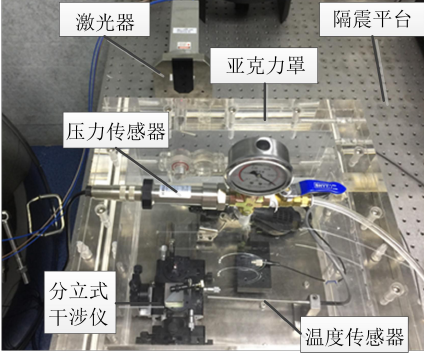
\includegraphics[width=7cm]{fig/1-fig/双频激光干涉仪环境误差补偿实验平台图.jpg}
  \caption{双频激光干涉仪环境误差补偿实验平台图}
  \label{fig:双频激光干涉仪环境误差补偿实验平台图}
\end{figure}

2022年,为解决PTF法对高精度传感器的依赖问题,浙江理工大学纳米测量技术实验室的严利平等人,提出了一种基于激光单频干涉和PTF传感融合的空气折射率测量方法,即使用低精度传感器获得低精度的空气折射率预测值,并以此确定干涉条纹的整数周期数;并在干涉仪测量臂上构建了两束测量光,分别经过真空腔内部和真空腔外部,并测量这两束测量光干涉的相位差即可得到相位的小数部分,并使用PGC-Arctan解调方法,以实现空气折射率的测量。实验设备如图\ref{fig:基于激光单频干涉和PTF传感融合的空气折射率测量装置图}所示\cite{2022基于激光单频干涉和PTF传感融合的空气折射率测量方法},主要包括激光器(ECDL)、PTF传感器、线性导轨滑块(GCD-040101M)、RedPitaya开发板以及Renishaw的空气折射率补偿单元(XC-80)。实验结果证明,与使用Edlen公式法得到的空气折射率测量结果相比,1小时内的标准偏差为2.3$\times 10^{-8}$。
\begin{figure}[htb]
  \centering
  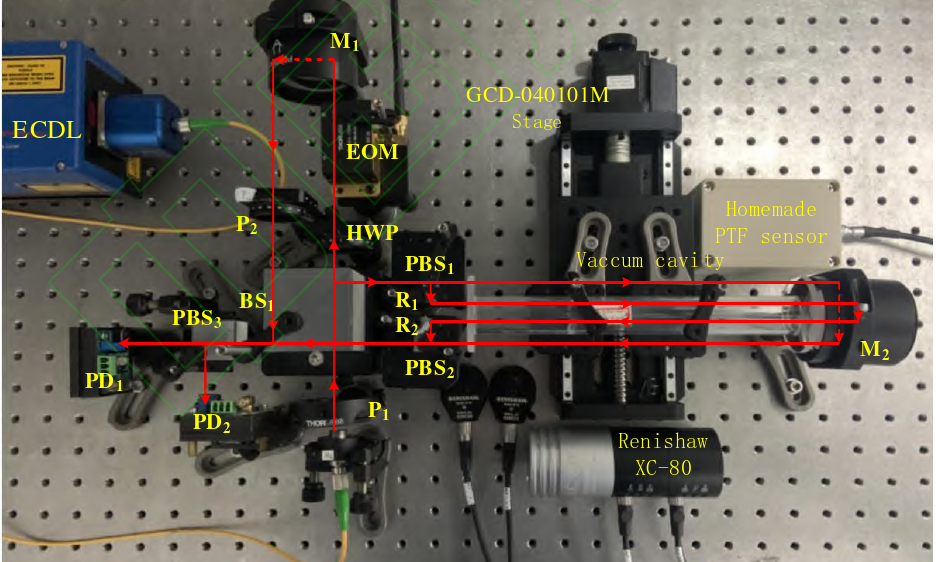
\includegraphics[width=11cm]{fig/1-fig/基于激光单频干涉和PTF传感融合的空气折射率测量装置图.png}
  \caption{基于激光单频干涉和PTF传感融合的空气折射率测量装置图}
  \label{fig:基于激光单频干涉和PTF传感融合的空气折射率测量装置图}
\end{figure}


\section{本文的主要工作及组织结构}
\subsection{本文的主要工作}
本文针对光刻机物镜可动机构的超精密位移的超高精度检测需求,开展基于双频激光干涉仪的精度的相关研究,而环境误差作为双频激光干涉仪的主要误差之一,是限制双频激光干涉仪测量精度的主要因素之一。本文结合使用Edlen公式和粒子群算法,从软件补偿和硬件补偿两个层面开展相关研究,主要包含以下研究内容:
\begin{enumerate}
    \item 实验系统的搭建、改进与实验测量。为了采样到更为精准的温度数据,开发了基于PT100温度传感器的多通道温度采集系统,基于LabVIEW开发了配套的上位机系统和标定系统,并且进行了标定过程,各通道的拟合优度值都大于0.9999。并且为了能够测量到精准的环境误差,从实验设备、实验变量、实验环境和实验方法等多个角度对实验系统进行了改进,例如为了减小材料热胀冷缩的影响,开发了一套环境误差测量专用的干涉仪,不含任何的金属外壳,而是使用光学元件直接粘接制成,并且将底座粘接在微晶玻璃上。在实验测量方面,为了保证补偿场景的完善性,进行了短时测量、长时测量以及大范围温度变化三种场景下的多次数据采集。
    \item 结合使用Edlen公式和粒子群算法进行补偿,以消除两种方法自身的局限性。现有的Edlen公式是根据644.0nm、508.7nm、480.1nm和467.9nm四个波长段在20$^{\circ}\mathrm{C}$测量数据得出的,而如今双频激光干涉仪的激光波长大多为633nm,并且光刻机中的工作温度为22$^{\circ} \mathrm{C}$,两者在波长段和使用温度上并不匹配。而粒子群算法当粒子群到达局部最优解附近时,粒子速度的更新主要由自身速度决定,这会使得粒子难以跳出当前的局部最优解,发生早熟收敛问题。将两者结合使用,以Edlen公式作为粒子群算法的搜索模型,能充分挖掘训练样本中的数据关系,解决Edlen公式条件不匹配问题,并且由于原始的Edlen公式为粒子群算法提供了一个优秀的搜索起点,相当于大幅压缩了粒子群算法的搜索空间,这能非常有效地避免早熟收敛问题的出现。
    \item 基于软件层面的补偿方法。使用整段式的粒子群算法补偿方法对实验数据进行补偿,补偿效果较未优化前的Edlen公式均得到了明显提升。但通过实验发现,传统的线性Edlen公式似乎并不适用于温度梯度变化较大的场景,为此进行了额外的实验,并且采用微积分的思想,在每一个极小的微分元内将非线性看成线性,提出了基于温度梯度的分段式粒子群算法补偿方法,实验证明该方法能够适用于温度梯度变化较大的场景。
    \item 基于硬件层面的加速补偿方法。基于温度梯度的分段式粒子群算法补偿方法的提出对粒子群算法的运算速度有着更高的要求,而提升运算速度的一大有效方法就是设计专用的加速结构。为此将软件层面的补偿算法进行了算法硬化,让其更加适合于硬件设计,并提出了双差分验证框架以保证硬件设计的正确性和可靠性。在设计过程中使用流水线技术提高系统吞吐率,并且设计了专用的流水线握手方案,针对粒子群算法的运算过程,设计专用的适应度计算模块、种群信息更新模块以及速度和位置更新模块对粒子群算法进行加速。
    \item 软硬件补偿方法的性能对比。软件补偿方法和硬件补偿方法各有优劣,通过真实的实验数据和仿真信息比较了两种方法在运行时间、硬件资源和补偿性能等方面的优劣,并对两种补偿方法进行了总结。
  \end{enumerate}
\subsection{本文的组织结构}
本文的研究工作主要分为七章,各章的主要安排如下:

第一章:绪论。本章首先会介绍课题的具体来源,论文的研究背景及意义,介绍国内外的研究人员在干涉仪环境误差补偿上所开展的相关研究工作,提出本文主要的研究内容,以及全文的章节架构。

第二章:双频激光干涉仪的环境误差及Edlen公式补偿方法。本章首先对激光位移测量理论基础进行了梳理,介绍了多普勒频移和拍频现象,并以此为基础扩展出单频激光干涉仪和双频激光干涉仪的测量原理,并从双频激光干涉仪的测量原理中推导出环境误差的成因和原理公式。随后介绍了Edlen公式,对公式的变化曲线进行了分析,并根据Edlen公式的诞生条件分析其局限性,为后续粒子群算法补偿方法的提出做了铺垫。

第三章:双频激光干涉仪的环境误差补偿实验系统。本章首先介绍了基于PT100的八通道温度测量系统的设计情况,包含其上位机软件的设计、标定程序的设计以及标定过程和标定结果,随后介绍了气压传感器以及补偿系统的总体方案,并从实验设备、实验变量、实验环境和实验方法四个方面对实验系统进行了多次改进,以便于测量到更加准确的环境误差。随后介绍了实验系统安装和调试过程,并采集了短时测量、长时测量以及大范围温度变化测量三种测量场景下的实验数据,使用原始的Edlen公式对实验数据进行补偿,验证了Edlen公式的补偿效果,便于后续工作开展时进行对比。

第四章:基于粒子群算法的软件补偿方法及算法硬化。本章首先介绍了粒子群算法的原理及算法过程,还有本文工作所使用的线性惯性权值递减策略。随后介绍基于粒子群算法优化后的Edlen公式补偿方法,包含数据预处理和训练过程。然后使用短时测量、长时测量以及大范围温度变化测量三种测量场景下的实验数据进行补偿,并与原始Edlen公式的补偿效果进行对比。但在实验过程中发现传统的线性Edlen公式似乎并不适用于温度梯度变化较大的场景,为此又开展了更多的实验,并使用微积分的思想,在每一个极小的微分元内将非线性看成线性,从而提出了基于温度梯度的分段式粒子群算法补偿方法,介绍了该方法的具体算法原理和流程图,并通过实验验证了算法的可行性。为了解决该方法对粒子群算法运行速度的高要求,将补偿算法进行算法硬化,主要包含:数据定点方案及截断方案、补码运算、乘除转换转换方案、四舍五入方案等,并在硬化过程中提出专用的差分验证环境,便于后续硬件设计工作的开展。

第五章:用于干涉仪环境补偿的粒子群算法的硬件加速补偿系统设计。本章首先介绍了在设计过程中使用到的流水线技术、握手控制技术、逻辑复制和资源共享技术、门控时钟技术以及基于线性反馈移位寄存器的随机数生成技术。然后介绍了粒子群算法加速补偿系统的总体架构,包含架构图、parameter定义表以及所有的接口信号表,并且分模块地介绍了适应度计算模块(pso$\_$fitness$\_$cal)、种群信息更新模块(pso$\_$population$\_$upda)以及速度和位置更新模块(pso$\_$velocity$\_$cal)三个模块的架构图和接口信号表。然后介绍了系统顶层的寄存器配置顺序以及多起点训练方法,最后提出双差分验证框架,即上述的差分验证框架中进行更新,引入硬件和算法硬化模型,在验证过程中进行两次验证。

第六章:软硬件补偿方法的性能对比。本章首先对比分析了软件补偿方法和硬件补偿方法的运行时间、资源消耗以及补偿效果,并对两种补偿方法的使用条件进行了总结。

第七章:总结和展望。本章主要是对全文的工作进行了总结,并对后续可能的研究方向进行了展望。

为了更加清晰地展示本文的组织结构,本文通过图\ref{fig:论文组织架构图}进一步展示各章节的内容和章节之间的脉络。

\clearpage
\begin{figure}[H]
    \centering
    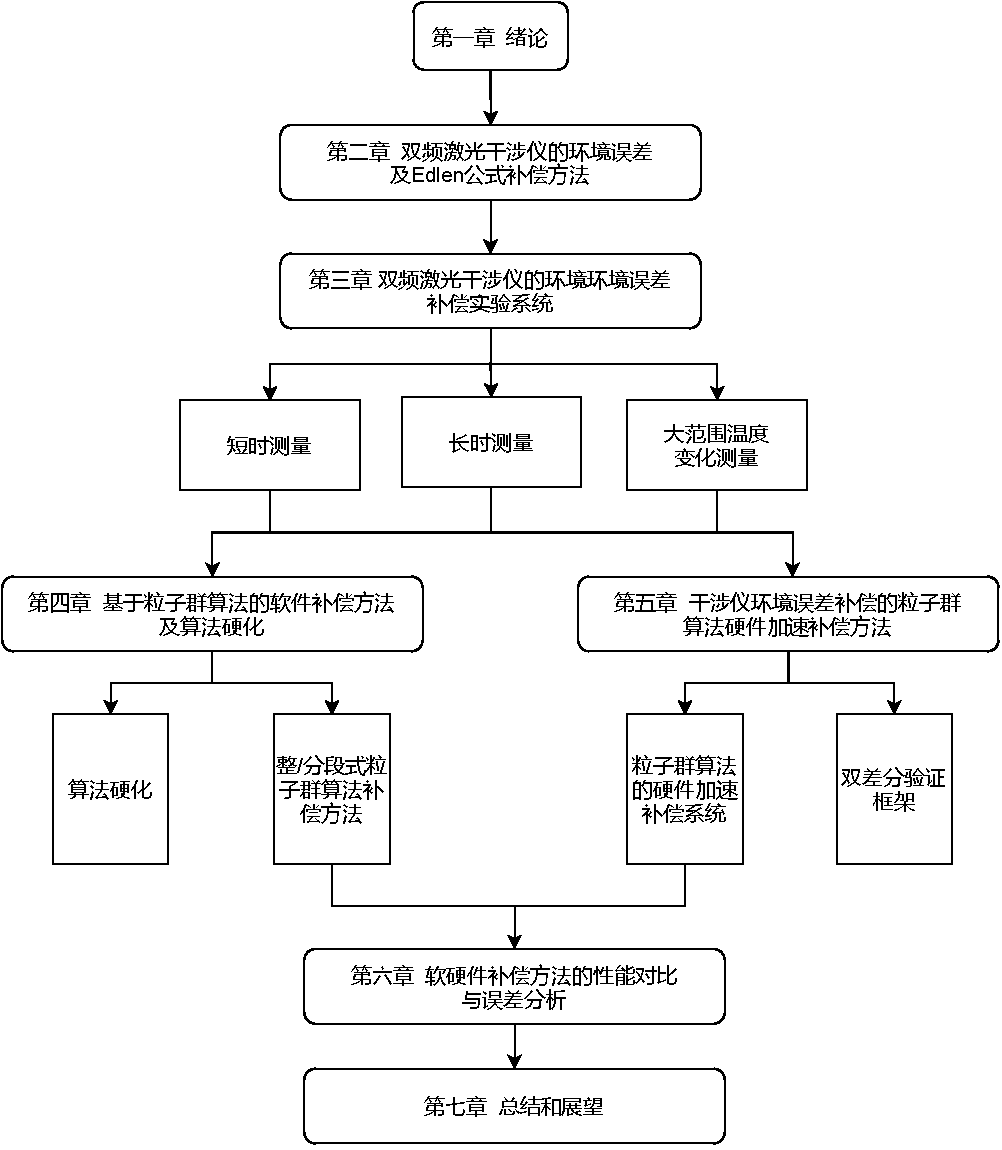
\includegraphics[width=13cm]{fig/1-fig/论文组织架构图.drawio.pdf}
    \caption{论文组织架构图}
    \label{fig:论文组织架构图}
\end{figure}